\section{Introduction}

%%%%%%%%%%%%%%%%%%%%%%%%%%%%%%%%%%%%%%%%%%%%%%%%%%%%%%%%%%%%%%%%%%%%%%%%%%%%
\subsection{Context}
\begin{frame}{Context: Embedded Systems and IoT}
	\begin{minipage}[c]{0.5\textwidth}
        \begin{block}{Internet of Things (IoT)}
            \begin{itemize}
                \setbeamertemplate{itemize items}[square]
                \justifying
                \item Wide range of application
                \item Fast growing market with exponential usage
                \item Rely on sensors depending on their use
                \item Collect and share data
                \item Manipulation of critical data
                \item Increasingly vulnerable to multiple threats
            \end{itemize}
        \end{block}
	\end{minipage}\hfill%
	\begin{minipage}[c]{0.5\textwidth}
		\begin{figure}
			\centering
			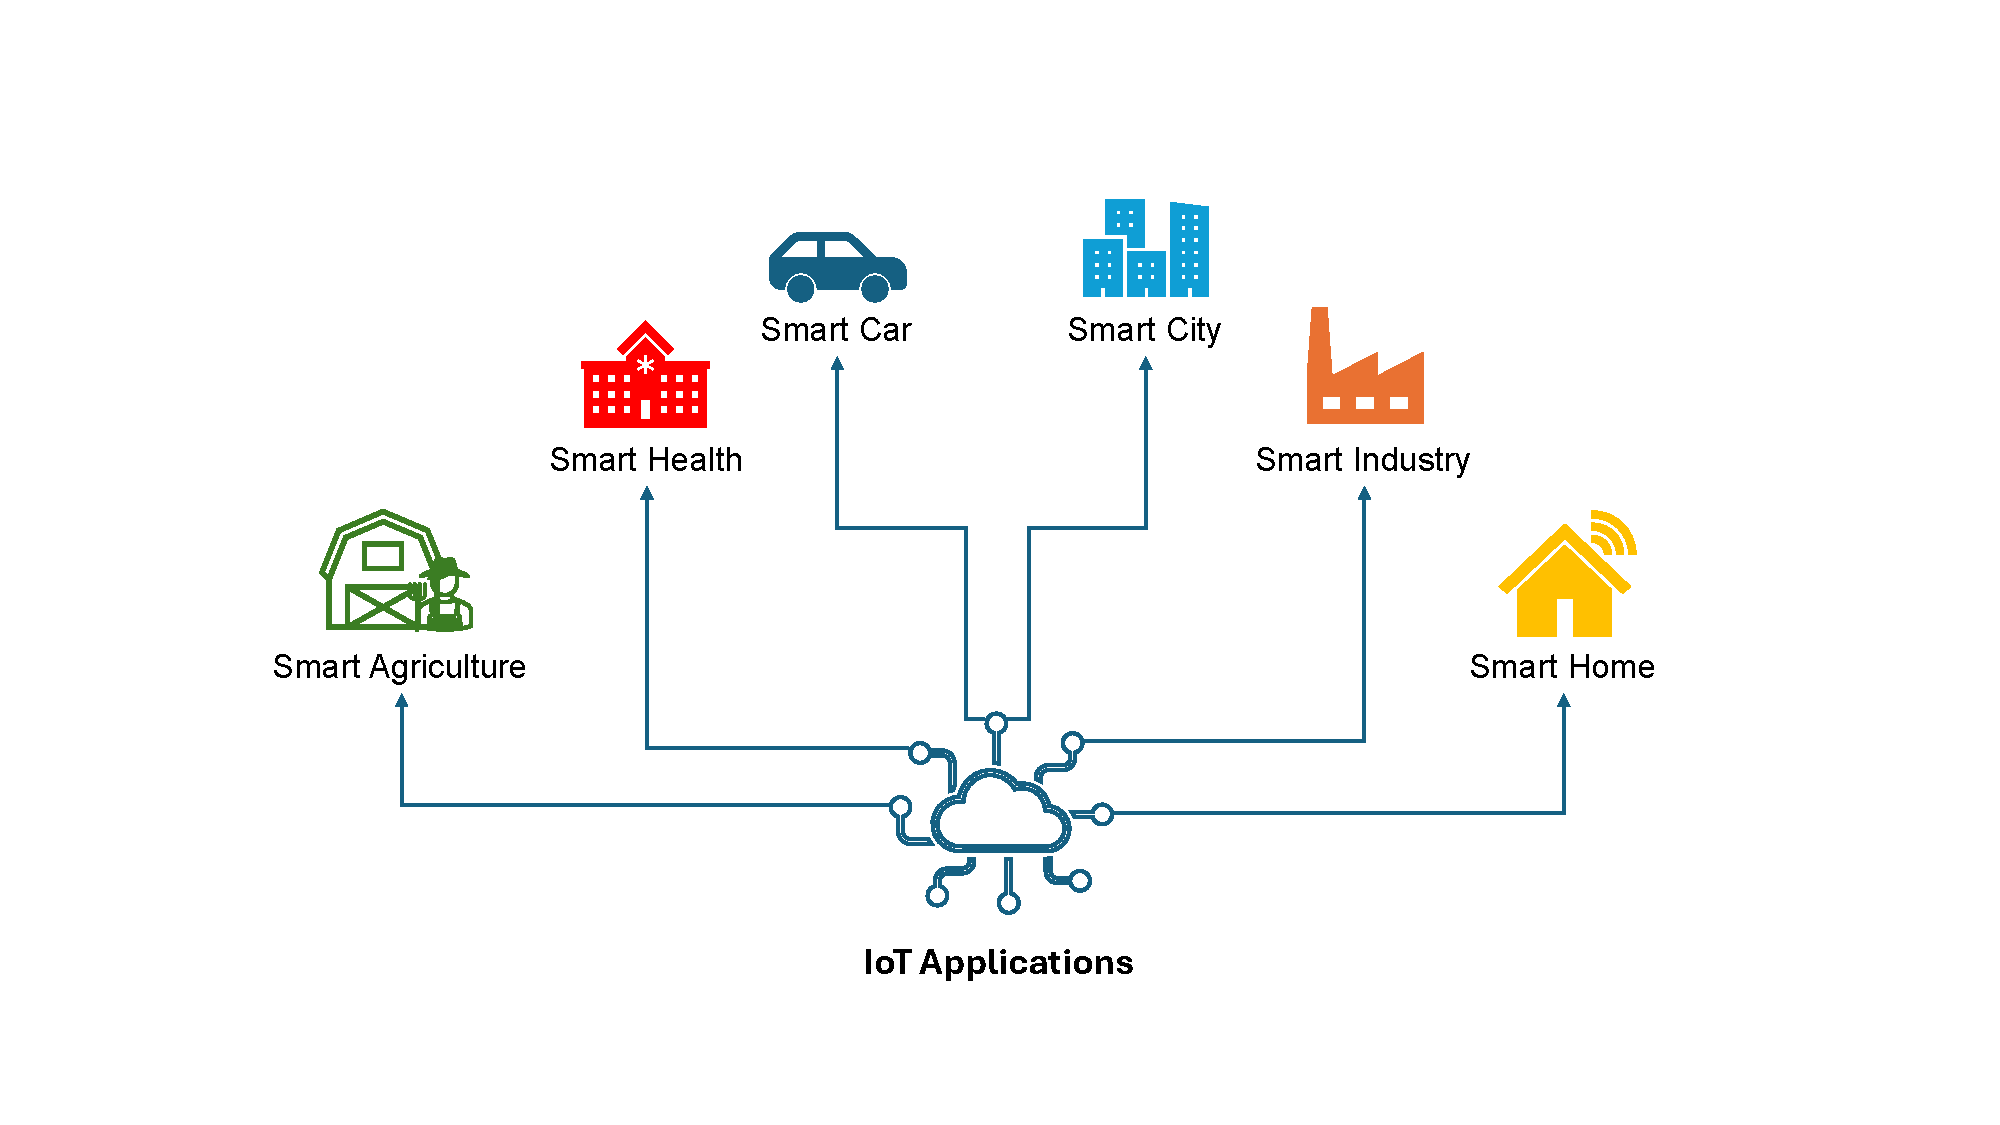
\includegraphics[width=.825\textwidth, trim={4.5cm 2.25cm 5.75cm 3.25cm}, clip]{src/1_introduction/img/iotapplications.pdf}
            % \caption{Example of IoT applications}
			\label{fig:iot_application}
		\end{figure}
        \vspace{-5pt}
        \begin{figure}
            \centering
            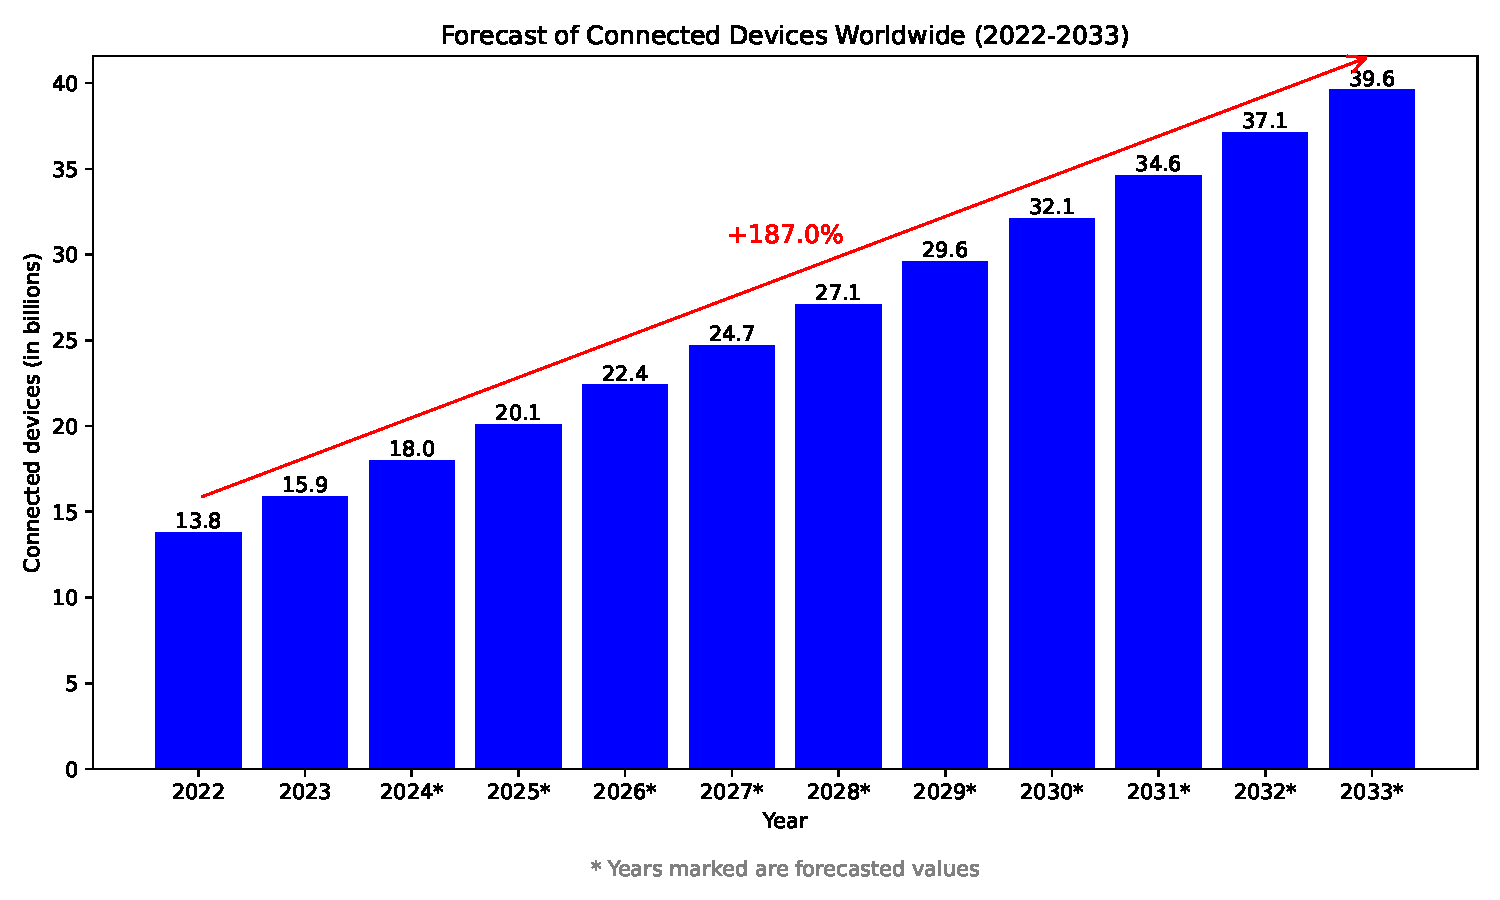
\includegraphics[width=.825\textwidth]{src/1_introduction/img/iot_forecasts.pdf}
            \label{fig:nbr_iot}
        \end{figure}
	\end{minipage}
\end{frame}

%%%%%%%%%%%%%%%%%%%%%%%%%%%%%%%%%%%%%%%%%%%%%%%%%%%%%%%%%%%%%%%%%%%%%%%%%%%%
\subsection{Motivations}
\begin{frame}{Motivations: IoT Under Threats}
    \only<1>{
        \begin{block}{Threats}
            \begin{itemize}
                \setbeamertemplate{itemize items}[square]
                \justifying
                \item Software threats: malwares, memory overflow attacks, SQL injection, etc
                \item Network threats: DDoS, Man-In-The-Middle, jamming, etc
                \item Hardware threats: physical attacks such as reverse engineering, Side-Channel Attacks (SCA), Fault Injection Attacks (FIA)
            \end{itemize}
        \end{block}
    }
    \only<2>{
        \begin{block}{Threats}
            \begin{itemize}
                \setbeamertemplate{itemize items}[square]
                \justifying
                \item \textbf{\textcolor{red}{Software threats}}: malwares, memory overflow attacks, SQL injection, etc
                \item Network threats: DDoS, man-in-the-middle, jamming, etc
                \item \textbf{\textcolor{red}{Hardware threats}}: physical attacks such as reverse engineering, Side-Channel Attacks (SCA), \underline{Fault Injection Attacks (FIA)}
            \end{itemize}
        \end{block}
    }

    \filigrane{A compléter}{45}{5}
\end{frame}
%%%%%%%%%%%%%%%%%%%%%%%%%%%%%%%%%%%%%%%%%%%%%%%%%%%%%%%%%%%%%%%%%%%%%%%%%%%%
\subsection{Software threats: Information Flow Tracking}
\begin{frame}{Software threats: Information Flow Tracking}
    \begin{block}{}
        \begin{itemize}
            \setbeamertemplate{itemize items}[square]
            \justifying
            \item Security mechanism
            \item Protection against software attacks (e.g.: \textit{buffer overflow}, \textit{format string}, \textit{SQL injections}, \ldots)~\cite{BSMCVEJCO-21-acmcsur, HAK-21-acmcsur}
            \item Static or \underline{Dynamic}
            \item Software, \underline{Hardware} or Hybrid
            \only<1>{\item \textcolor{Gainsboro}{Hardware DIFT: off-core, off-loading core, in-core}}
            \only<2->{\item Hardware DIFT:} \only<2>{\textbf{off-core}, \textcolor{Gainsboro}{off-loading core, in-core}}\only<3>{off-core, \textbf{off-loading core}, \textcolor{Gainsboro}{in-core}}\only<4>{off-core, off-loading core, \underline{\textbf{in-core}}}
        \end{itemize}
    \end{block}
    

    \only<2>{
        \begin{figure}
            \centering
            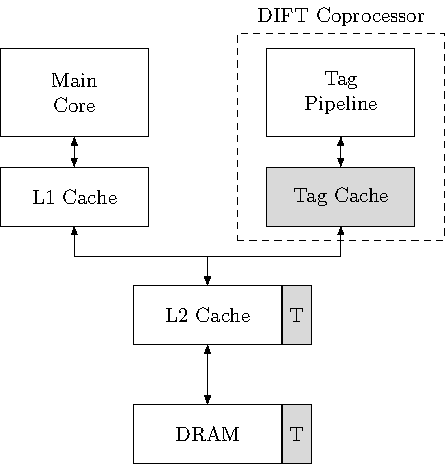
\includegraphics[height=.5\textheight]{src/1_introduction/img/offcore.pdf}
            \label{fig:offcore}
        \end{figure}
    }
    \only<3>{
        \begin{figure}
            \centering
            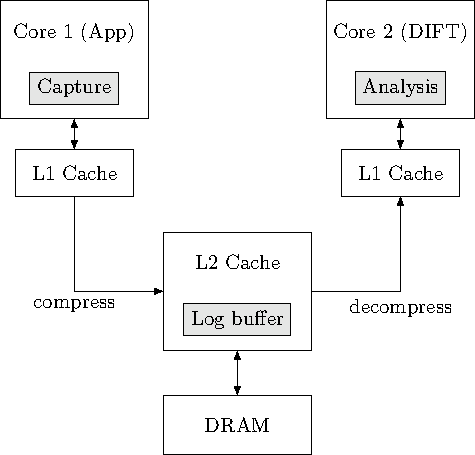
\includegraphics[height=.5\textheight]{src/1_introduction/img/offloading.pdf}
            \label{fig:offloading}
        \end{figure}
    }
    \only<4>{
        \begin{figure}
            \centering
            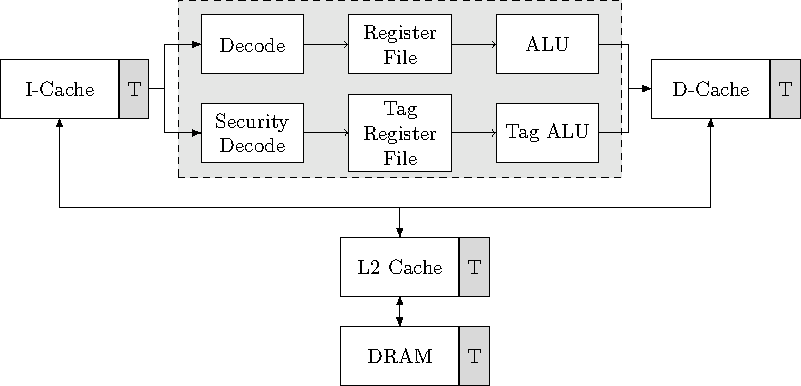
\includegraphics[height=.5\textheight]{src/1_introduction/img/incore.pdf}
            \label{fig:incore}
        \end{figure}
    }
\end{frame}

\begin{frame}{Dynamic Information Flow Tracking}
    \begin{minipage}[c]{0.35\linewidth}
        \begingroup
        \begin{block}{\textbf{Three} steps}
            \begin{itemize}
                \item<1-> Tag initialisation
                \item<2-> Tag propagation
                \item<3-> Tag check
            \end{itemize}
        \end{block}
        \endgroup
    \end{minipage}\hfill%
    \begin{minipage}[c]{0.6\linewidth}
        \begin{figure}
            \centering
            \only<1>{\includegraphics<1>[width=1\textwidth, page=1]{src/1_introduction/img/schemaDIFT.pdf}}
            \only<2>{\includegraphics<2>[width=1\textwidth, page=2]{src/1_introduction/img/schemaDIFT.pdf}}
            \only<3->{\includegraphics<3->[width=1\textwidth, page=3]{src/1_introduction/img/schemaDIFT.pdf}}
            \label{fig:schemaDIFT}
        \end{figure}
    \end{minipage}
\end{frame}
%%%%%%%%%%%%%%%%%%%%%%%%%%%%%%%%%%%%%%%%%%%%%%%%%%%%%%%%%%%%%%%%%%%%%%%%%%%%
\subsection{Hardware threats: Physical Attacks}
\begin{frame}{Hardware threats: Physical Attacks}
    \begin{block}{}
        \begin{itemize}
            \setbeamertemplate{itemize items}[square]
            \justifying
            \item<1> Reverse Engineering: process of information retrieval from a product by analysing and understanding the design, functionality, and operation of existing hardware
            \item<2> Side-Channel Attacks: exploit information leakages on the circuit behaviour
            \item<3> \underline{Fault Injection Attacks}: involve deliberately introducing one or more fault(s) into the system to observe its behaviour and identify potential vulnerabilities.
        \end{itemize}
    \end{block}

    \only<2>{
        \begin{figure}
            \centering
            \includegraphics[height=.5\textheight, page=3]{src/1_introduction/img/physicalAttacks.pdf}
            \label{fig:sca}
        \end{figure}
    }

    \only<3>{
        \begin{figure}
            \centering
            \includegraphics[height=.5\textheight, page=2]{src/1_introduction/img/physicalAttacks.pdf}
            \label{fig:fia}
        \end{figure}
    }
\end{frame}
%%%%%%%%%%%%%%%%%%%%%%%%%%%%%%%%%%%%%%%%%%%%%%%%%%%%%%%%%%%%%%%%%%%%%%%%%%%%
\subsection{Issue}
\begin{frame}{Issue}
    \begin{exampleblock}{}
        How can we maintain maximum protection against software attacks in the presence of physical attacks?
    \end{exampleblock}
\end{frame}
%%%%%%%%%%%%%%%%%%%%%%%%%%%%%%%%%%%%%%%%%%%%%%%%%%%%%%%%%%%%%%%%%%%%%%%%%%%%
\subsection{Objectives}
\begin{frame}{Objectives of this PhD Thesis}
    \begin{block}{Contributions}
        \begin{itemize}
            \setbeamertemplate{itemize items}[triangle]
            \justifying
            \item Provide a robust security mechanism against software and hardware threats.
            \item Take into account Fault Injection Attacks
            \item Propose lightweight countermeasures against FIA
            \item Take into account constraints, such as area and performance overhead
        \end{itemize}
    \end{block}
\end{frame}
%%%%%%%%%%%%%%%%%%%%%%%%%%%%%%%%%%%%%%%%%%%%%%%%%%%%%%%%%%%%%%%%%%%%%%%%%%%%